\chapter{Background and Concepts}
In this chapter, we will introduce several main concepts related to our study.
\section{Agile software development}
\label{agile}
The term "Agile" represents the fast adaptation and response to the changes \cite{highsmith2002agile}.
Agile software development is a new method of software development that implements the ideology of "agile". Agile software development advocates the continuous development of software teams. The software development under this methodology will have shorter planning/development time before it delivers to the costumers and could better adapt to changes in the environment and requirements.
\paragraph{Iterative Software Development:} Agile software development uses an iterative way in the development process. The traditional software development process, like the waterfall method, requires the long and complicated planning process, and a complicated document. Once one phase of the development is done, the teams shouldn't change the output (document and code) of this phase \cite{cusumano1995beyond}. In contrast, the agile software development aims to satisfy the customer with early and continuous delivery of the software \cite{beck2001manifesto}. Early means the shorter time before software delivery. Continuous means the development does not end with the delivery. Delivery means the end an iteration, together with a demonstration to stakeholders. After delivery, the team continue to next iteration according to the feedback it gets from stakeholders. In each iteration, the team not aims to add major features to the software, rather their goal \cite{beck1999embracing} is to have a working and deliverable release. In the ideology of agile, the best design the software product comes from the iterative development \cite{beck2001manifesto}, rather than the tedious planning.
\paragraph{High Software Quality:} The rapid development doesn't mean low software development quality. On the contrast, the quality of software design is highly appreciated in the agile software development. The automatic testing is widely used in Agile. The test cases will be defined and implements from the beginning of the development process. The testing goes through the whole development iteration ensure the software has a high enough quality to be released or demonstrate to costumers at any point of an iteration \cite{Agilesof32:online}.
\paragraph{Collaboration:}
The agile software development processes include collaboration across different groups, ie. bushiness development team, software development team, test team, and costumers. It values more face to face communications \cite{beck2001principles} and feedbacks. The goal for these communications is, firstly to let everyone in the multifunctional agile team understand the whole project, secondly, to receive feedback that helps the software in the right development track that aligns with the requirement of the stakeholders \cite{beck2001manifesto}. 
\par
According to the Manifesto for Agile Software Development, compared with traditional software development, the agile software development value these aspects \cite{beck2001manifesto}: 
\begin{itemize}
\item Individuals and interactions over processes and tools.
\item Working software over comprehensive documentation.
\item Customer collaboration over contract negotiation.
\item Responding to change over following a plan.
\end{itemize}
\section{Continuous Integration \& Continuous Delivery}
In the software development, CI/CD refers to continuous integration, continuous delivery and continuous deployment \cite{pittet2018continuous}. As we mentioned in \ref{agile}, agile software development requires continuous software quality assurance and iterative development. Currently, CI/CD is one set of the necessary practices for the team to become agile by achieving the requirements above. Figure \ref{fig:cicd} shows the relationship between these 3 practices.
\begin{figure}[h]
    \centering
    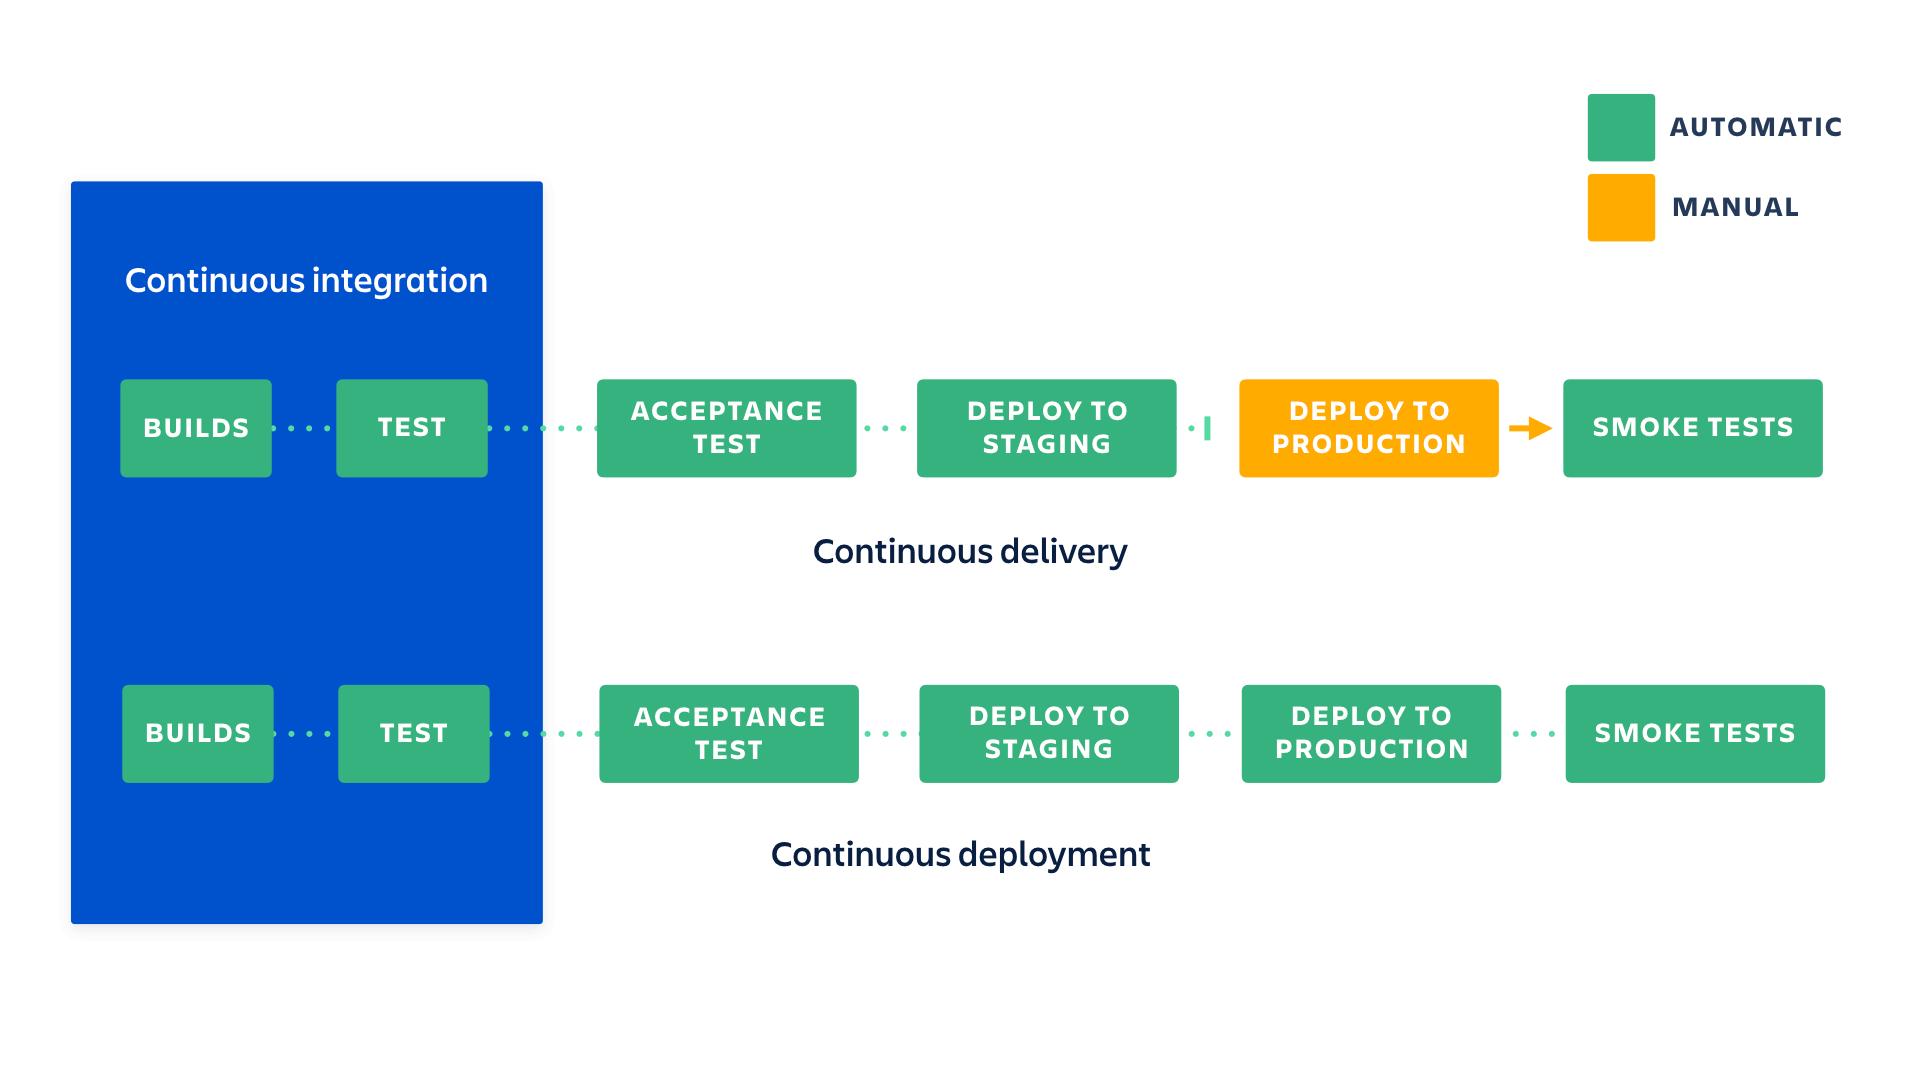
\includegraphics[width=0.95\textwidth]{pics/cicd.png}
    \caption{The relationship between continuous integration, continuous delivery and continuous deployment \cite{pittet2018continuous}}
    \label{fig:cicd}
\end{figure}
\subsection{Continuous Integration}
Continuous interaction is the base practice of all practices within CI/CD, and continuous delivery/deployment is based on the continuous interaction \cite{pittet2018continuous}.
The continuous integration means the team integrate each team member's work into main codebase frequently(multiple times per day). "Integrate" means merge the code to the main codebase \cite{fowler2006continuous}. The continuous interaction rely on 2 practices: \textit{Build Automation} and \textit{Test Automation}. The definition of these 2 practices are:
\begin{itemize}
    \label{TestA}
    \item \textit{Test Automation:} Test automation means using separate software to execute the software automated, without human intervention. It could help the team to test fast and test early \cite{Testauto48:online}. 
    \item \textit{Build Automation:} Automate the process of creating software build. This means to automate the dependency configuration, source code compiling, packaging and testing. It is viewed as the first step to continuous integration \cite{Buildaut62:online}.
\end{itemize}
With the help of these 2 practices, for each developer in the team, the workflow \cite{fowler2006continuous} in continuous interaction as follows: In the development of each feature, the developer first pull the code from the main codebase. During the development, new test cases could also be added to the automated test. After the development is done, automated testing also runs on the code to maintain the code quality and minimize the number of bugs from the beginning. The build automation compiled the code locally in the development machine. 
\par
After the step above, the developer already has the executable and the high quality (passed the automated test) code in the development machine before submitting the change to the code base. This represents the principle of quality and automation in agile software development. In the next step, the developer commits changes to the repository, which is the main codebase, and the system check the conflict and do the test/build again, to make sure that there are not any bugs missed in the test on the development machine.
If the code passes this build and test, it will be merged to the main codebase and the integration is done.
\subsection{Continuous Delivery and Continuous Deployment}
\label{CD}
Continuous delivery is practices that software development team build a software that can be released at any time of the lifecycle.\cite{fowler2013continuous}This means the software always maintains a high quality and in a deployable state\cite{WhatisCo47:online}. It is a subset of agile, which focuses on the software delivery\cite{Continuo97:online}. From the last section, we introduce the concept of continuous interaction. The continuous delivery is based on continuous interaction but further automate the software deployment pipeline. In the software deployment pipeline, the team divide build into several stages, first build the product and then push the product into the production-like environment for further testing. This ensures that the software could be pushed to production at any time. However, in continuous delivery, the deployment of software into production is done manually.
The benefit \cite{WhatisCo47:online}\cite{fowler2013continuous} of continuous delivery includes:
\begin{itemize}
    \item High code quality: The automate and continuous testing ensure the quality of the software.
    \item Low risk: The software could be related at any time, and it's easier to release and harder to make the mistake
    \item Short time before going to the market: The iteration of software development is much shorter. The automation in testing, deployment, environment confirmation included in the process, and the always read-to-deploy status shorten the time from development to market.
\end{itemize}
The continuous deployment is based on continuous delivery. The only difference is continuous deployment automates the deployment process. In continuous delivery, the software is deployable but not deploy without manual approval. In the continuous deployment, each change that passed automated build and testing will be deployed directly. The continuous deployment is a relatively new concept that most company not yet put the practice into production \cite{leppanen2015highways}. While continuous delivery is the required practice for the company to be DevOps and it is already being widely used.
\section{DevOps}
\begin{quotation}
    The fundamental goal of DevOps is to minimize the service overhead so that it can respond to change with minimal effort and deliver the maximum amount of value during its lifetime.
    \begin{flushright}
        -- Markus Suonto, Senior DevOps Consultant, Eficode
    \end{flushright}
\end{quotation}
\subsection{Definition}
\label{devops}
DevOps is a set of practices that aims to combine different, traditionally separated disciplines (eg. software development, operations, QA, and others) in cross-functional teams with the help of automation of work to speed up software delivery without risking high-quality \cite{bass2015devops}.
\par
DevOps is the extension and evolution \cite{lwakatare2016relationship}\cite{leite2019survey} of Agile. DevOps and Agile both driven by the collaboration ideology and the adoption of DevOps needs Agile as the key factor \cite{lwakatare2016relationship}. DevOps has a different focus on agile. DevOps focus on the delivery while agile is focused on the development with the requirement and customer. Figure \ref{fig:DevOps} shows the workflow and practices of a team working under DevOps.
\begin{figure}[h]
    \centering
    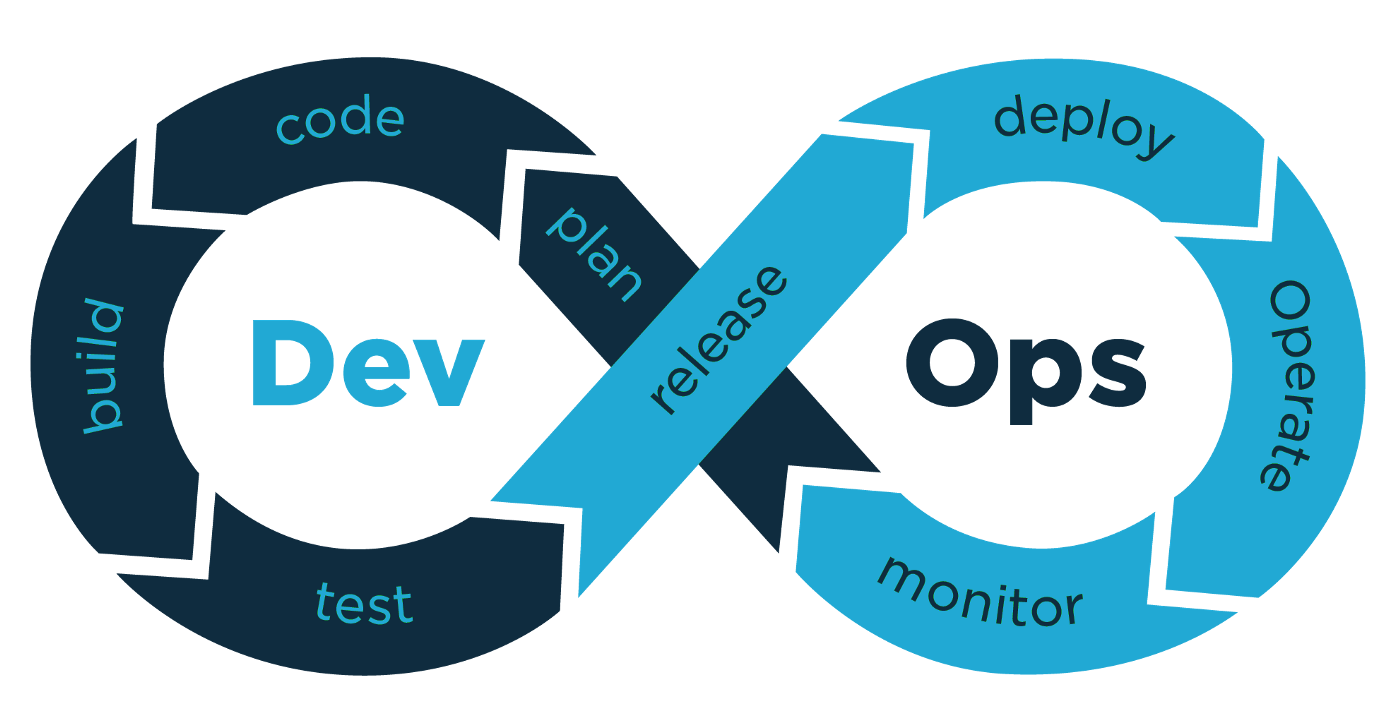
\includegraphics[width=0.95\textwidth]{pics/DevOps.png}
    \caption{DevOps Practices and Workflow \cite{DevOpsin72:online}}
    \label{fig:DevOps}
\end{figure}
\subsection{Elements}
In this section, we will introduce the necessary elements that an organization need to includes when employing DevOps. 4 necessary elements need to be considered.
\subsubsection[]{Culture}
In the pre-DevOps era, the Development and Operation are two different teams with a different goal. The interface between them is based on the ticket system which the operation team do the ticket management. As we mentioned at \ref{agile}, the goal of Agile is to shorten the deliver life cycle and delivery software quickly to the costumers. So when practice agile development method under this scenario, the development try to deliver the code they develop earlier but the operation team usually will delay the process for quality control or other reasons. In practice, this causes the delay between the code change and the software delivery to the costumers \cite{leite2019survey}. 
The lack of communication and conflict between developers and the operation team slow down the software delivery process and also make it harder for the teams to be real Agile. Therefore the concept "DevOps" is being proposed at 2008, for eliminating of the boundary between developers (Dev) and operation team (Ops). According to Walls (2013), this is being done by promoting the culture with 4 characterises: open communication, incentive and responsibility alignment, respect and trust \cite{walls2013building}.
\par 
The open communication means openly discussion and debate. As mentioned above, the traditional communication method is through a very formal and regularized ticket system. In the DevOps, the communication is not limited within the formal ticket system. instead, the team will keep in the whole lifecycle of a product, from the requirement, schedule, and anything else. \cite{walls2013building} The information sharing is also important \cite{lwakatare2015dimensions}. The metrics and the project status is available for everyone in the team \label{moniter}, so each member could have a clear scope about what the team is doing.
\par
The incentive and responsibility alignment mean the whole teams (combines Dev and Ops) shares the same goals and also takes the same responsibility. The shift from "Dev" and "Ops" to DevOps requires people who used charges in only development and operation starting sharing the responsibility from both side \cite{lwakatare2015dimensions}. This means individuals or a certain part of the team will be not solely blamed if the product is failed. This "no blame" culture could help each engineer be willing to take the development responsibility for the whole system \cite{feitelson2013development}.
\par 
Respect means all employees should respect and recognize the contribution of other teams members. A DevOps team is not a single team without any division of jobs, there is still an operation part within a team \cite{TheresNo86:online}. However the people operation team will take development responsibility, and the developers will also put their hands-on operation and management\cite{shropshire2017uncertainty}. To make people with different roles works in a team, trust and respect each other is critically important. 
\subsubsection[]{Organisation}
In the organizational level, the DevOps emphasizes the collaboration between different part of an organization. This is strongly correlated with the "culture" part of this section. Inside a team, each member should be a generalist who could understand all aspect of a project. There will not be a dedicate QA, operation or security team within a team. Instead, these are the job that belongs to everyone \cite{feitelson2013development}\cite{kim2016devops}. The organization should provide the team member with opportunities to learn all skill needed for building the whole system. 
\par
The team size should be small. A small team could help to reduce the inter-team communication. The small team means the scope of the project is small. And it also means less bureaucracy in team management. There are four benefits \cite{kim2016devops} to have a small team:
\begin{itemize}
    \item The smaller team allows each team member to easily understand the whole project.
    \item The smaller team could reduce the amount of communication needed. It could also limit the growth rate that the product could have.
    \item The smaller team could decentralize power. In DevOps, each team lead could define the metrics which become the overall criteria of the whole team's performance.
    \item In a smaller team, failure doesn't mean a disaster for the company. This allows the team to fail. Thus each employee could train their headship skill in the team without too much pressure. 
\end{itemize} 
\par
Furthermore, another important organizational aspect for DevOps is to have a loosely-coupled architecture. 
The first benefit of this is the better safety.
In the organisation with a tightly-coupled architecture, small changes could result in large failure \cite{kim2016devops}.
The second benefit is productive. In a traditional organisation, the result of each team will be merged, tested together and deploy together. This means it is time-costly to configure and manage the test environment requires dependencies. A loose organisation enable each team to finish the development of lifecycle (from planing to deployment) independently. Each team could update their products independently, which gives the team more flexibly to align the product with the change in the customer requirement. This means the update of each team's product won't affect other teams as well.
\subsubsection[]{Automation}
In the DevOps, automation means 
automation within the whole development and operation process. The organisations which employing DevOps aims for a high degree of automation\cite{erich2017qualitative}.
With automation, people could be free from the repetitive work and reduce human error. It could help build the DevOps culture of collaboration, and it is seen as the cornerstone of the DevOps \cite{DevOpsCu76:online}.
The main practices regarding Automation are the automated testing, continuous delivery and automated operation. Automated testing could be achieved by test automation. We already mentioned the benefit of this at \ref{TestA}.
\par
The continuous delivery pipeline is the core of the DevOps \cite{gill2018devops}. As we discussed at \ref{CD}. The continuous delivery will ultimately automate all steps between the developer to commit the code to the product in the production.
\par
\label{iasc}
The automation of the operation part is usually done by using the concept of "Infrastructure as Code" \cite{lwakatare2015dimensions}. The Infrastructure as Code (IasC) means to define everything in the software infrastructure level as code \cite{artac2017devops}. Because it is code, we could use the automation methodology used in the software development to manages and deploy these codes. According to Christof et. (2016), under IasC, infrastructure can be shared, tested, and version controlled \cite{ebert2016devops}. This could help emphasizes the automation within the operation scope. With the automation in operation, the team could be free from the tedious environment configuration and shorten the product development lifecycle. Automating server configuration means the developers and operation staff can equally know the server configuration \cite{DevOpsCu76:online} which help build the culture of shared responsibility and trust.
\subsubsection[]{Monitoring and Measurement}
Monitoring is to continuously collect the matrices from the running system for helping the team find the problems in the system. To do the monitoring, the monitoring system need to do measurement, which is to collect data properly from the system. The measurement be defined as reducing the uncertainty through observation, which producing quantitative result \cite{hering2015measure}. The result (metrics) should be properly used by the organisation.
\par
In the DevOps way of development, the testing is the key to maintain the quality of the software continuously. However, when the product enters the production, we cannot test the software any more. So, we need monitoring to keep track the status of the product \cite{huttermann2012devops}. According to State of DevOps report from Google, the good monitoring structure and the wisely usage of the data from monitoring for making bushiness decision could improve the software delivery performance \cite{forsgrenaccelerate}. Thus, Monitoring is an important component of DevOps.
\par
With monitoring, the software team could keep tracking the status, and maintain the quality of deployed production. The monitoring has also enabled the team to collect the data from costumers' usage behaviour. This helps the agile development team to make an improvement in the next iteration of the product \cite{lwakatare2015dimensions}.
\par
For develop a high-quality monitoring system, the development of monitoring could be in parallel with the main product, and the monitoring system can be already be used against the "staging deployment" (see Figure \ref{fig:cicd}) at the early stage of the iteration. By this, the development team can improve the monitoring system continuously together with the main software system. The parallel development of the monitoring system and the main system helps the team to find the gap in the monitoring earlier \cite{huttermann2012devops}.
\par
As we mentioned in the "Culture" section, the collaboration is an important part of the DevOps culture. collaboration needs the communication and information sharing between the development(Dev) and operation(Ops) team. The monitoring could be one of the channels between the Dev and Ops since it can expose the information of the whole system which helps team members to understand the system as a whole. This helps the team achieving the point we mentioned at \ref{moniter} (Culture) that the project status and matrices should available to every team members.
\subsection{Toolchain}
A DevOps toolchain is a set of tools that integrated together to aid the software development, deployment and management through the whole software development lifecycle, which helps the software development to fit the DevOps principles \cite{DevOpsto7:online}\cite{Toolchai10:online}\cite{WhatisaD20:online}. Each tool in the toolchain supports on specific activities in DevOps, for example, version control, build, testing.
\par
According to \cite{WhatisaD20:online}, Google Cloud state of DevOps reports \cite{forsgrenaccelerate}\cite{velasquez2014state}\cite{forsgren20192019} and our previous definition of the DevOps, we summarize the essential component of a DevOps toolchain as below.
\subsubsection{Project Management \& Planning}
Planning software development project, track the tickets and the issues, communication between and within the teams. The project management tools help to implement the DevOps culture, which enhances collaboration and knowledge sharing.\\
\textbf{Tools:} Slack, Jira, Trello, Asana
\subsubsection{Configuration Management}
Provided a central platform to manage the configuration across the assets. This usually done by defining the desired state of the assets in a configure file and automate the configuration process which reaching the assets to the defined status.\\
\textbf{Tools:} Puppet, Chef, Ansible
\subsubsection{Continuous Integration}
Continuous integration (in short: CI) is the top practice for improving the Deployment Frequency \cite{velasquez2014state}. It is one of the most important parts of DevOps toolchain. As we introduced at \ref{CD}, CI allows the developers to integrate their work more frequently to the production products, it shortens the time to the market of the product. The automatic testing and code analysis integrated into the CI continuously maintain the quality of the product. CI tools also automated the most parts of the software development pipeline, In conclusion, CI helps the system fulfil the DevOps definition (\ref{devops}) by speed up the delivery by automation, maintain the quality by continuous quality assurance. So CI is the core part of the whole DevOps toolchain.\\
\textbf{Tools:} Jenkins, Drone CI, Teamcity, GitLab CI/CD
\subsubsection{Version Control}
Version control is the key component of DevOps toolchain. It is a system that could record and track the changes in a set of file overtime. Version control simplifies the collaboration between team members. and allow the simultaneous development on the different part of a software system According to \cite{Sourcean53:online} and \cite{velasquez2014state}, version control is the top practices when comes to improve the multiple metrics in DevOps. Version control becomes the indicator of the software system performance \cite{Sourcean53:online} Infrastructure as code, an important DevOps practise we mentioned at \ref{iasc} also relies on the version control.\\
\textbf{Tools:} GitHub, Gitlab, Bitbucket
\subsubsection{Monitoring}
The monitoring system is one of the basic practices in a DevOps toolchain\cite{forsgren20192019}. It is also one of 4 basic elements of DevOps as we mentioned at \ref{moniter}. In the DevOps toolchain, the monitoring system detect the failure in the whole system and helps the software team finds the problems earlier. The log taking by the monitoring system can also record the system activity history which allows the further analysis.\\
\textbf{Tools:} Zabbix, Promethus
\subsubsection{Automated Testing}
The automated testing tool could verify the code before it being build. Due the common practise of continuous integration which we mentioned at \label{CD}, the automated testing usually integrated in the continuous integration pipeline. The integration of testing in CI pipeline makes it easy for organisation to implement the quality gate in the software development \cite{huttermann2012devops}.
\\
\textbf{Tools:} Robot Framework, Selenium, JMeter

\section{Serverless Computing}
In this section we focus on the concepts of Serverless Computing.


We will have more discussion regarding to new cloud service based on Serverless Computing in the next chapter.

